\documentclass[tikz,convert={outfile=figure1_timeline.png}]{standalone}
\usepackage{pgfplots}
\pgfplotsset{compat=1.18}
\begin{document}
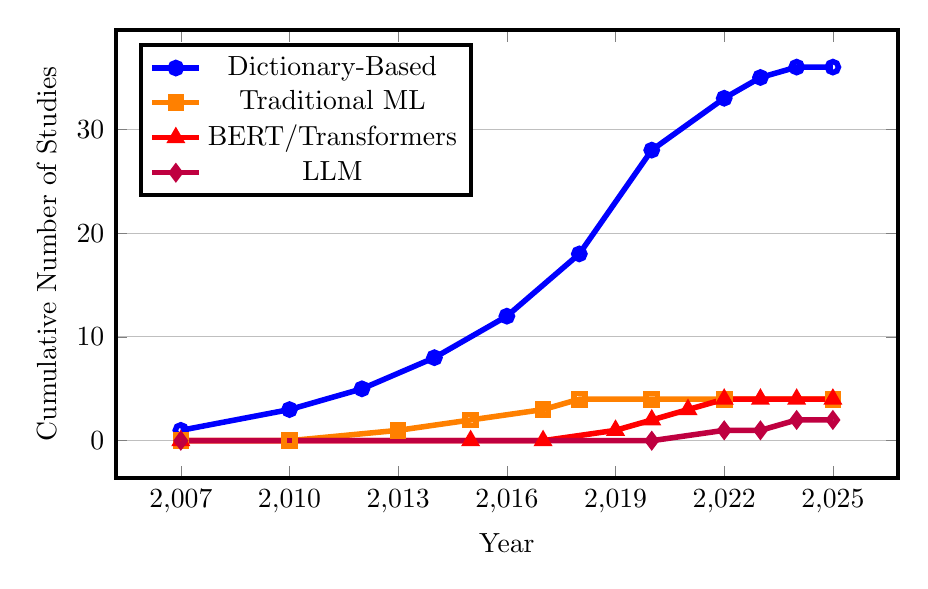
\begin{tikzpicture}
\begin{axis}[
    width=0.95\textwidth,
    height=0.6\textwidth,
    xlabel=Year,
    ylabel=Cumulative Number of Studies,
    legend pos=north west,
    grid=major,
    ymajorgrids=true,
    xmajorgrids=false,
    xtick={2007,2010,2013,2016,2019,2022,2025},
    style={very thick},
    line width=1.5pt,
]
\addplot[mark=o, color=blue, line width=2pt] coordinates {
    (2007, 1) (2010, 3) (2012, 5) (2014, 8) (2016, 12) (2018, 18) (2020, 28) (2022, 33) (2023, 35) (2024, 36) (2025, 36)
};
\addlegendentry{Dictionary-Based}
\addplot[mark=square, color=orange, line width=2pt] coordinates {
    (2007, 0) (2010, 0) (2013, 1) (2015, 2) (2017, 3) (2018, 4) (2020, 4) (2022, 4) (2025, 4)
};
\addlegendentry{Traditional ML}
\addplot[mark=triangle, color=red, line width=2pt] coordinates {
    (2007, 0) (2015, 0) (2017, 0) (2019, 1) (2020, 2) (2021, 3) (2022, 4) (2023, 4) (2024, 4) (2025, 4)
};
\addlegendentry{BERT/Transformers}
\addplot[mark=diamond, color=purple, line width=2pt] coordinates {
    (2007, 0) (2020, 0) (2022, 1) (2023, 1) (2024, 2) (2025, 2)
};
\addlegendentry{LLM}
\end{axis}
\end{tikzpicture}
\end{document}
